\section{Early stage researchers}
\label{esrs}
12 ESRs form the core of the network, with the training and partnerships providing a scaffold for the completion of their respective outcomes. Each ESR is enrolled as a doctoral student at a partner university for 3 years, during which they complete secondments in HEP and industry, as illustrated in Figure~\ref{esr-diagram}. The university of enrolment is generally also the hosting institution, where the majority of the doctoral study is completed (industry-centred ESR positions are enrolled at a university near to the respective industry partner). A secondment in HEP is undertaken either at another partner university or a partner research institute. Each ESR (with the exception of those in industry-centred positions) also undertakes a secondment in industry, working on an RTA project relevant to their research with an industry partner.

\begin{figure*}[h!]
    \centering
    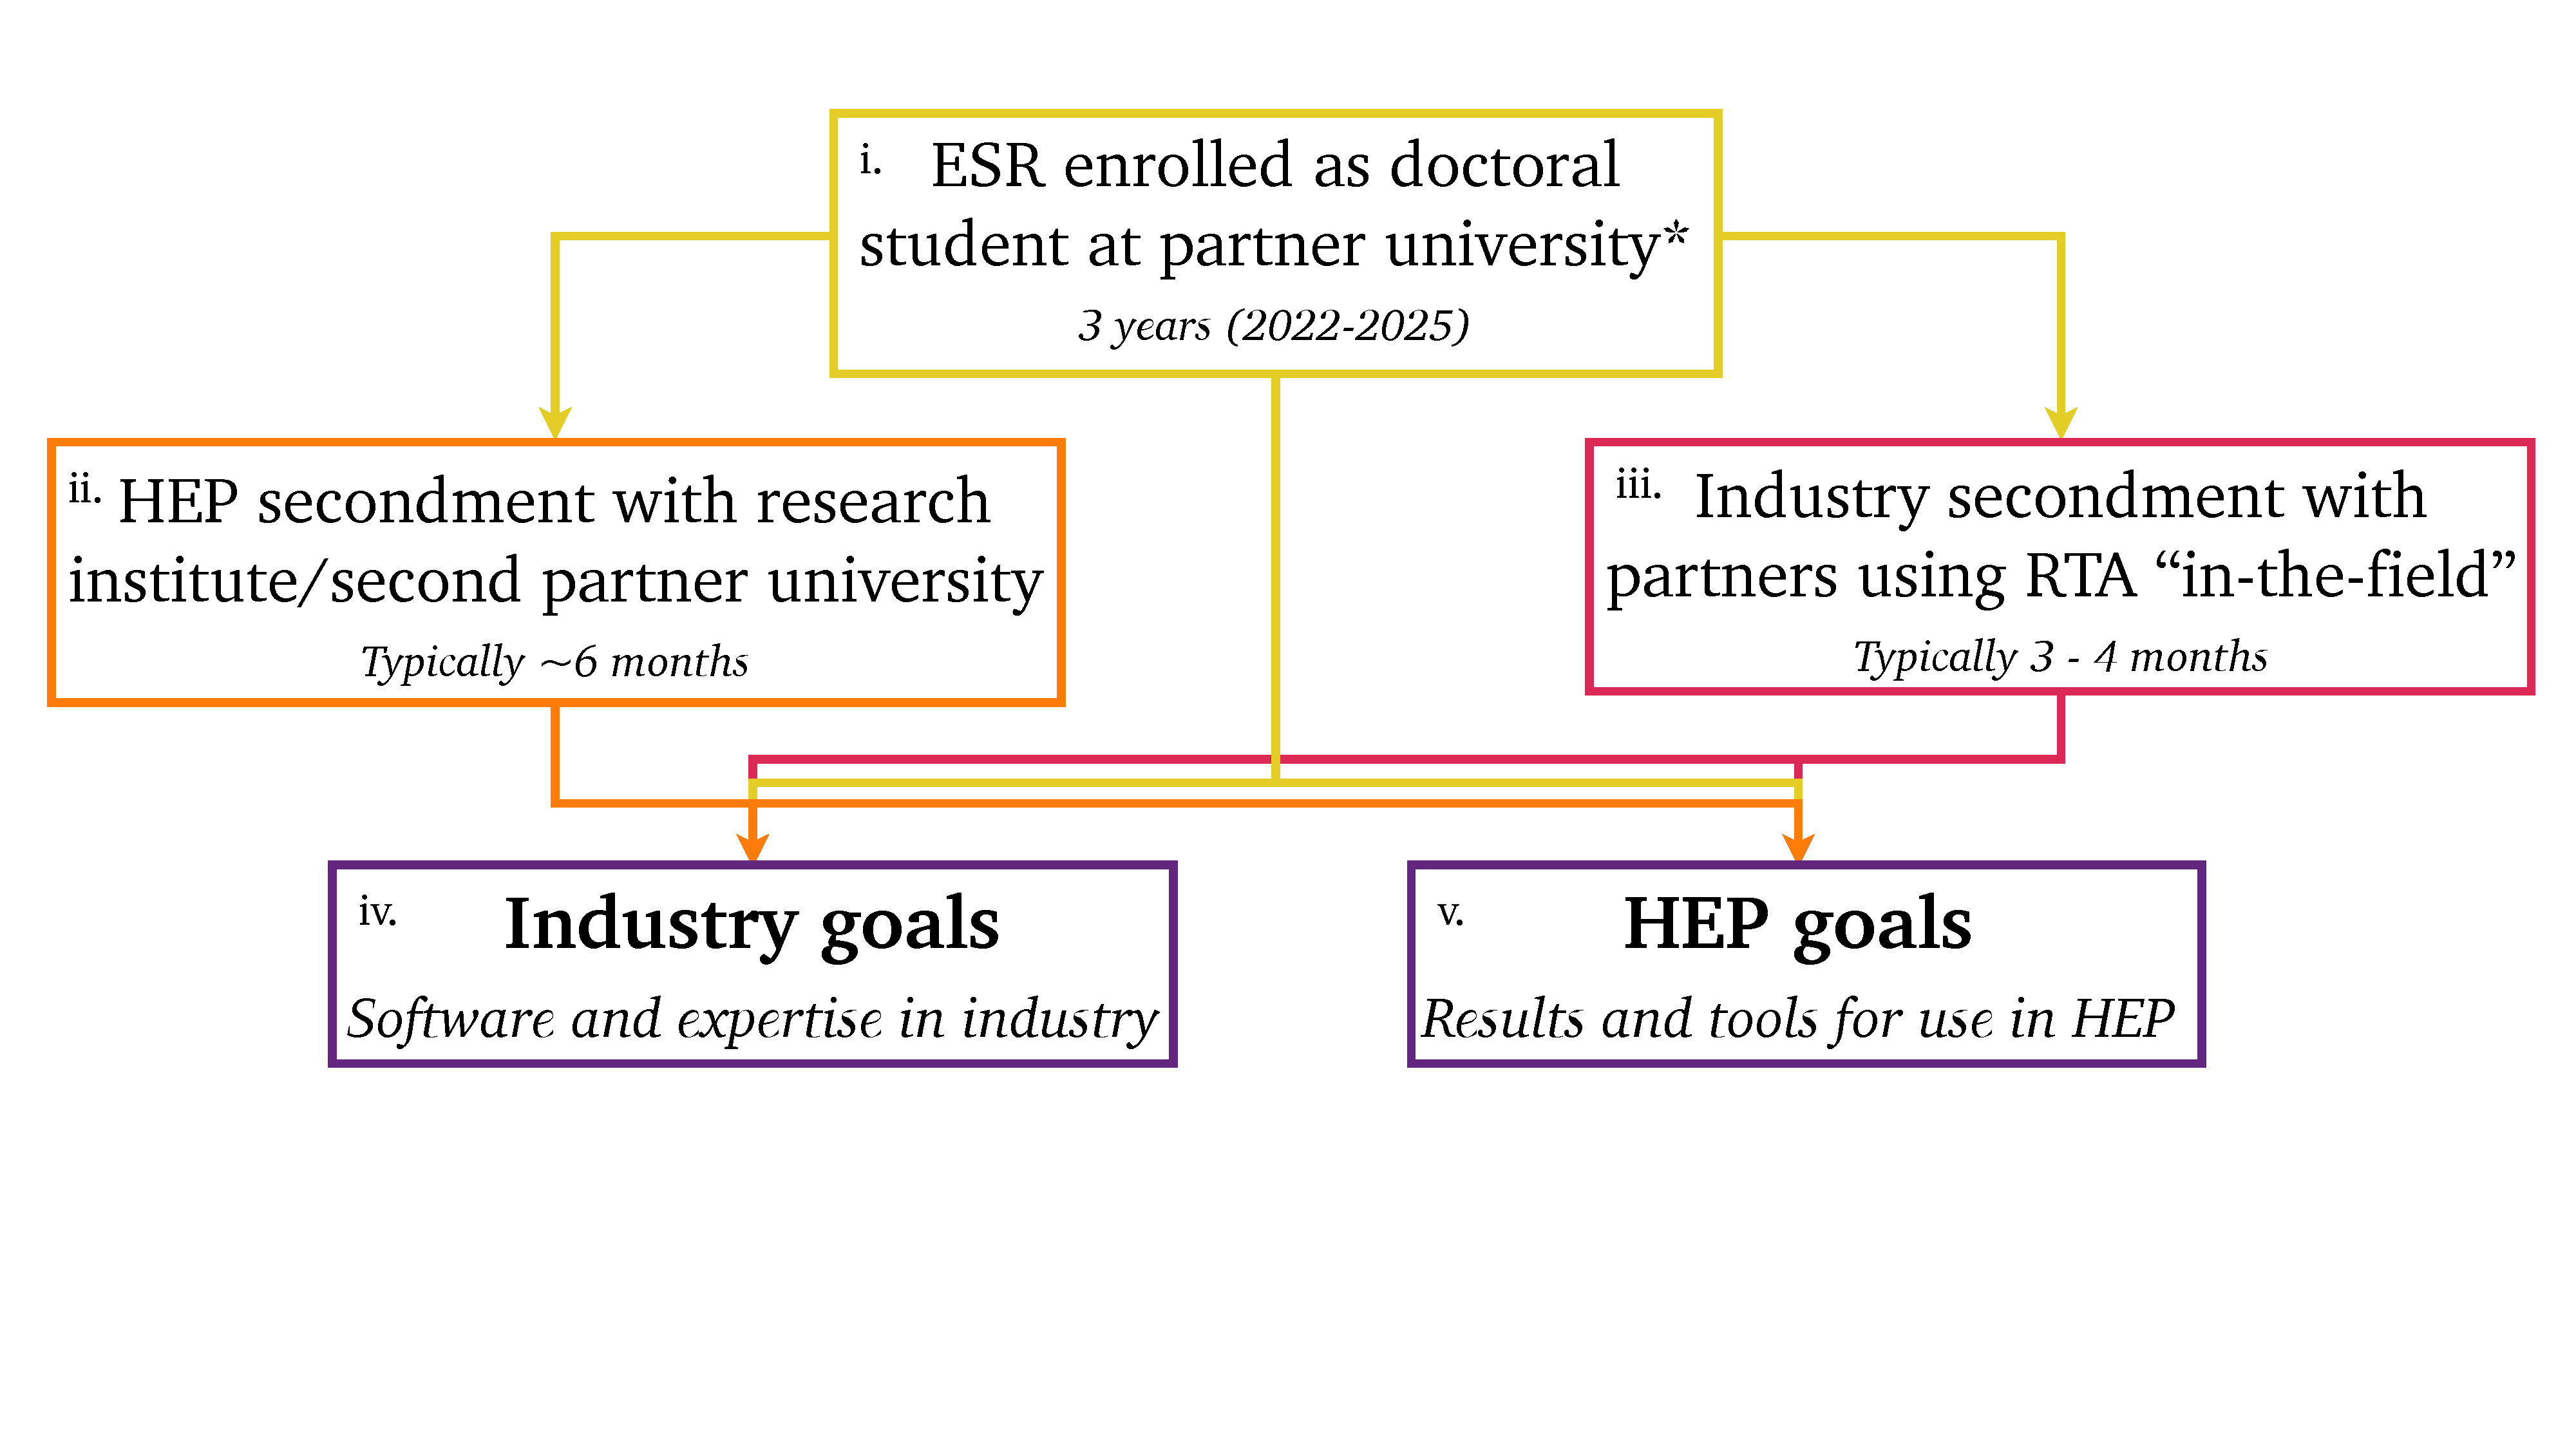
\includegraphics[width=\linewidth]{/Users/jgooding/Documents/SMARTHEP/CHEP2023/CHEP2023/proceedings/figures/esr-diagram.pdf}
    \caption{Structure of a SMARTHEP ESR position. Each ESR is enrolled (i.), during which they will undertake secondments with network partners in HEP (ii.) and industry (iii.). Through the combination of primary and secondment work, each ESR will complete goals in HEP (iv.) and industry (v.), discussed in further detail in Section~\ref{outcomes}. Precise durations of the secondments vary between ESR positions.}
    \label{esr-diagram}
\end{figure*}

To illustrate further the structure of a SMARTHEP ESR position, academia- and industry-centred examples are given below. Details of the positions are given alongside their corresponding label in Figure~\ref{esr-diagram}.

Firstly, an example of an academia-centred position is the ESR based at the University of Heidelberg (i.). Their primary focus is working on real-time searches for Dark Photons at LHCb (iv.), furthered by collaboration with the University of Milano-Bicocca (ii.). An industry secondment (iii.) with Verizon Connect is planned, applying ML expertise to the real-time processing of vehicle data (v.). 

An industry-centred position is well-typified by the ESR working at IBM, enrolled at Sorbonne University (i.). Their research applies real-time rule induction to fraud detection using real-time rule induction at IBM (v.). An industry secondment (iii.) is not undertaken, since the primary research is undertaken with an industry partner; however, an academic secondment (ii.) is planned with the CNRS research institute, applying similar pattern-recognition techniques to the classification of HEP observations (iv).
